\documentclass{article}
% if you need to pass options to natbib, use, e.g.:
%     \PassOptionsToPackage{numbers, compress}{natbib}
% before loading neurips_2023
\usepackage[final]{neurips}
% to avoid loading the natbib package, add option nonatbib:
%    \usepackage[nonatbib]{neurips}


\usepackage[utf8]{inputenc} % allow utf-8 input
\usepackage[T1]{fontenc}    % use 8-bit T1 fonts
\usepackage{hyperref}       % hyperlinks
\usepackage{url}            % simple URL typesetting
\usepackage{booktabs}       % professional-quality tables
\usepackage{amsfonts}       % blackboard math symbols
\usepackage{nicefrac}       % compact symbols for 1/2, etc.
\usepackage{microtype}      % microtypography
\usepackage{xcolor}         % colors
\usepackage{graphicx}       % include graphics
\usepackage{subcaption}     % subfigures
\usepackage{amsmath}        % math environments
\usepackage{algorithm}      % algorithm environment
\usepackage{algorithmic}    % algorithmic pseudo-code


\title{Predicting Canadian Dollar Exchange Rates Against Major Global Currencies Using Machine Learning}


\author{%
  Xi Chen\\
  Department of Electrical \& Computer Engineering\\
  University of Toronto\\
  \texttt{xialex.chen@mail.utoronto.ca} \\
  \And
  Xuhui Zhang\\
  Department of Electrical \& Computer Engineering\\
  University of Toronto\\
  \texttt{xuhui.zhang@mail.utoronto.ca} \\
  \And
  Wenxi (John) Chen\\
  Department of Electrical \& Computer Engineering\\
  University of Toronto\\
  \texttt{wxi.chen@mail.utoronto.ca} \\
}

\begin{document}


\maketitle


\begin{abstract}
We study next-business-day prediction of the Canadian dollar (CAD) exchange rate against three major currencies---USD, EUR, and CNY---using daily data from the Bank of Canada. The task is formulated as supervised regression with 22 engineered features (lagged values, rolling statistics, returns, and cyclical date encodings). We compare a persistence forecast, ordinary least-squares linear regression, support vector regression (SVR) with grid-searched hyperparameters, a multilayer perceptron (MLP), and a long short-term memory (LSTM) network. The persistence forecast achieves the best test performance on all three pairs, narrowly exceeding linear regression and showing that high level-prediction $R^2$ values are largely driven by strong day-to-day autocorrelation. MLP and LSTM remain competitive on EUR/CAD and CNY/CAD, whereas tuned SVR performs poorly on USD/CAD. We analyze the role of autocorrelation, target normalization, and robust time-series validation.
\end{abstract}

\section*{Attestation of Teamwork}
All three team members contributed equally to all stages of this project, including problem formulation, model design and implementation, experimentation, and report writing.


\section{Introduction}

Exchange-rate forecasting is a central problem in computational finance, supporting hedging, trade pricing, and policy analysis~[1]. The Canadian dollar is of particular interest because Canada is a major trading partner of the United States, the European Union, and China. Traditional econometric approaches such as the random-walk model remain difficult-to-beat baselines~[2], but advances in machine learning have renewed interest in data-driven forecasting, with nonlinear models showing promise on financial time series~[3,~4].

We investigate whether supervised learning methods can identify predictive structure in daily CAD exchange-rate data against three currencies (USD, EUR, CNY), comparing them with a persistence forecast that predicts the next rate as the latest observed rate.


\section{Preliminaries and Problem Formulation}

\subsection{Problem Setting}

We consider the task of predicting the next-day exchange rate of the Canadian dollar against a target currency. Let $r_t$ denote the exchange rate on business day $t$. Given a feature vector $\mathbf{x}_t \in \mathbb{R}^d$ constructed from historical observations up to and including day $t$, we seek a function $f: \mathbb{R}^d \rightarrow \mathbb{R}$ such that:
\begin{equation}
  \hat{r}_{t+1} = f(\mathbf{x}_t)
\end{equation}
where $\hat{r}_{t+1}$ is the predicted exchange rate for day $t+1$.

\subsection{Feature Construction}

The feature vector $\mathbf{x}_t$ consists of 22 engineered features derived from the raw exchange-rate time series:

\begin{itemize}
  \item \textbf{Lag features}: $r_{t-k}$ for $k \in \{1, 2, 3, 5, 7, 10, 14, 21\}$, providing the model with recent price history at multiple time scales.
  \item \textbf{Rolling statistics}: The rolling mean $\bar{r}_{t}^{(w)}$ and rolling standard deviation $\sigma_{t}^{(w)}$ computed over windows $w \in \{5, 10, 21, 50\}$ business days (shifted by one day to avoid look-ahead bias).
  \item \textbf{Percentage changes}: The 1-day and 5-day returns, $\Delta r_t^{(1)} = (r_t - r_{t-1})/r_{t-1}$ and $\Delta r_t^{(5)} = (r_t - r_{t-5})/r_{t-5}$.
  \item \textbf{Cyclical date encodings}: Sine and cosine transformations of the day-of-week ($\sin(2\pi d/5)$, $\cos(2\pi d/5)$) and month ($\sin(2\pi m/12)$, $\cos(2\pi m/12)$) to capture calendar seasonality without introducing ordinal artifacts.
\end{itemize}

\subsection{Evaluation Metrics}

We evaluate model performance using three standard regression metrics:
\begin{align}
  \text{MAE} &= \frac{1}{n}\sum_{i=1}^{n} |r_i - \hat{r}_i| \\
  \text{RMSE} &= \sqrt{\frac{1}{n}\sum_{i=1}^{n} (r_i - \hat{r}_i)^2} \\
  R^2 &= 1 - \frac{\sum_{i=1}^{n}(r_i - \hat{r}_i)^2}{\sum_{i=1}^{n}(r_i - \bar{r})^2}
\end{align}
where $r_i$ and $\hat{r}_i$ are the actual and predicted values, $\bar{r}$ is the mean of the actual values, and $n$ is the number of test samples.

	
\section{Design}

Our system follows a modular pipeline design consisting of five stages, as illustrated in Figure~\ref{fig:pipeline}.

\begin{figure}[!t]
  \centering
  \fbox{%
    \parbox{0.9\textwidth}{\centering
      \textbf{Data Download} $\rightarrow$ \textbf{Feature Engineering} $\rightarrow$ \textbf{Train/Val/Test Split} $\rightarrow$ \textbf{Model Training} $\rightarrow$ \textbf{Evaluation \& Visualization}
    }%
  }
  \caption{High-level pipeline architecture.}
  \label{fig:pipeline}
\end{figure}

The pipeline comprises five modules: (1)~\textbf{Data Loader} loads daily data from the Bank of Canada Valet API for USD/CAD, EUR/CAD, and CNY/CAD (2017--2025; 2,244 observations each); (2)~\textbf{Preprocessing} constructs 22 features (Section~2.2), performs a chronological 70/15/15 split, and applies standard scaling to both features and targets (fitted on the training set only); (3)~\textbf{Models} implements a persistence forecast, Linear Regression, SVR with grid-searched hyperparameters (scikit-learn), MLP, and LSTM (PyTorch); (4)~\textbf{Training} handles fitting with early stopping for the MLP and LSTM, and grid search for SVR; (5)~\textbf{Evaluation} computes metrics and generates figures.


\section{Methodology}

\subsection{Persistence Baseline}

Exchange rates are often well approximated over short horizons by a random walk. We therefore include a persistence forecast,
\begin{equation}
  \hat{r}_{t+1} = r_t,
\end{equation}
which uses the latest observed rate as the next-business-day prediction. A learned model should improve on this baseline to demonstrate predictive value beyond level autocorrelation.

\subsection{Linear Regression}

Ordinary least-squares (OLS) linear regression serves as our baseline. The model assumes a linear relationship between features and the target:
\begin{equation}
  \hat{r}_{t+1} = \mathbf{w}^\top \mathbf{x}_t + b
\end{equation}
where $\mathbf{w} \in \mathbb{R}^d$ and $b \in \mathbb{R}$ are learned by minimizing the sum of squared residuals. We use the \texttt{LinearRegression} class from scikit-learn~[5].

\subsection{Support Vector Regression (SVR)}

SVR finds a function that deviates from the training targets by at most $\varepsilon$ while remaining as flat as possible~[6]. We use the radial basis function (RBF) kernel:
\begin{equation}
  K(\mathbf{x}_i, \mathbf{x}_j) = \exp\!\left(-\gamma \|\mathbf{x}_i - \mathbf{x}_j\|^2\right)
\end{equation}
Hyperparameters are selected via grid search over $C \in \{0.1, 1, 10, 100\}$, $\varepsilon \in \{0.001, 0.01, 0.1\}$, and $\gamma \in \{\text{scale}, \text{auto}\}$ (24 combinations), evaluated on validation-set RMSE. The implementation uses the \texttt{SVR} class from scikit-learn.

\subsection{Walk-Forward Validation}

The reported experiment uses one chronological training/validation/test split. A more robust extension is walk-forward validation. At fold $k$, the model is trained only on observations available up to time $t_k$ and evaluated on the immediately following block satisfying $t_k < t \leq t_{k+1}$. The training window then moves forward---either expanding from the original start date or rolling with a fixed width---and the process repeats. Metrics are aggregated across the validation blocks, so hyperparameters must perform across multiple market regimes rather than one favorable interval. This procedure preserves temporal order and closely simulates deployment because future observations never enter training. After hyperparameter selection, the model can be refit on the combined training and validation period and evaluated once on the untouched final test set. Walk-forward validation is described here as recommended future methodology and is not used for the numerical results below.

\subsection{Multilayer Perceptron (MLP)}

The MLP is a feedforward neural network implemented in PyTorch~[7]. The architecture consists of three hidden layers with 128, 64, and 32 neurons respectively. Each hidden layer applies the following sequence of operations:

\begin{equation}
  \mathbf{h}^{(l)} = \text{Dropout}\!\Big(\text{ReLU}\!\big(\text{BatchNorm}(\mathbf{W}^{(l)} \mathbf{h}^{(l-1)} + \mathbf{b}^{(l)})\big)\Big)
\end{equation}

The output layer is a single linear neuron producing the scalar prediction $\hat{r}_{t+1}$.

\begin{algorithm}[!t]
\caption{MLP Training with Early Stopping}
\label{alg:mlp}
\begin{algorithmic}[1]
\REQUIRE Training data $(\mathbf{X}_{\text{train}}, \mathbf{y}_{\text{train}})$, validation data $(\mathbf{X}_{\text{val}}, \mathbf{y}_{\text{val}})$, patience $P$
\STATE Initialize MLP parameters $\theta$
\STATE $\text{best\_loss} \leftarrow \infty$, $\text{counter} \leftarrow 0$
\FOR{epoch $= 1, 2, \ldots, E_{\max}$}
  \FOR{each mini-batch $(\mathbf{X}_b, \mathbf{y}_b)$ from training set}
    \STATE $\hat{\mathbf{y}}_b \leftarrow \text{MLP}_\theta(\mathbf{X}_b)$
    \STATE $\mathcal{L} \leftarrow \text{MSE}(\hat{\mathbf{y}}_b, \mathbf{y}_b)$
    \STATE $\theta \leftarrow \theta - \eta \nabla_\theta \mathcal{L}$ \COMMENT{Adam optimizer}
  \ENDFOR
  \STATE Compute $\mathcal{L}_{\text{val}}$ on validation set
  \IF{$\mathcal{L}_{\text{val}} < \text{best\_loss}$}
    \STATE $\text{best\_loss} \leftarrow \mathcal{L}_{\text{val}}$, save $\theta^*$, $\text{counter} \leftarrow 0$
  \ELSE
    \STATE $\text{counter} \leftarrow \text{counter} + 1$
  \ENDIF
  \IF{$\text{counter} \geq P$}
    \STATE \textbf{break} \COMMENT{Early stopping}
  \ENDIF
\ENDFOR
\RETURN $\theta^*$
\end{algorithmic}
\end{algorithm}

\textbf{Training details:} The MLP is trained using the Adam optimizer~[8] with learning rate $\eta = 10^{-3}$, weight decay $10^{-5}$, batch size 64, and a maximum of 200 epochs. A \texttt{ReduceLROnPlateau} scheduler halves the learning rate if validation loss does not improve for 10 epochs. Early stopping with patience $P = 20$ epochs prevents overfitting. Dropout rate is set to 0.2.

\subsection{Long Short-Term Memory Network (LSTM)}

The LSTM~[10] is a recurrent architecture designed to capture temporal dependencies in sequential data. Unlike the MLP, which processes each sample independently, the LSTM receives a sliding window of $L = 21$ consecutive feature vectors as input, allowing it to learn patterns across time steps.

At each time step $t$, the LSTM cell computes:
\begin{align}
  \mathbf{f}_t &= \sigma(\mathbf{W}_f [\mathbf{h}_{t-1}, \mathbf{x}_t] + \mathbf{b}_f) & \text{(forget gate)} \\
  \mathbf{i}_t &= \sigma(\mathbf{W}_i [\mathbf{h}_{t-1}, \mathbf{x}_t] + \mathbf{b}_i) & \text{(input gate)} \\
  \mathbf{o}_t &= \sigma(\mathbf{W}_o [\mathbf{h}_{t-1}, \mathbf{x}_t] + \mathbf{b}_o) & \text{(output gate)} \\
  \mathbf{c}_t &= \mathbf{f}_t \odot \mathbf{c}_{t-1} + \mathbf{i}_t \odot \tanh(\mathbf{W}_c [\mathbf{h}_{t-1}, \mathbf{x}_t] + \mathbf{b}_c) \\
  \mathbf{h}_t &= \mathbf{o}_t \odot \tanh(\mathbf{c}_t)
\end{align}
where $\sigma$ is the sigmoid function and $\odot$ denotes element-wise multiplication.

Our LSTM uses 2 stacked layers with hidden size 64 and dropout 0.2 between layers. The final hidden state $\mathbf{h}_L$ of the last layer is passed through a linear output layer to produce the scalar prediction $\hat{r}_{t+1}$. Training uses the same Adam optimizer, learning rate scheduler, and early stopping strategy as the MLP.

\textbf{Libraries:} We use Python 3.11, PyTorch 2.0+ for the MLP and LSTM, scikit-learn 1.3+ for Linear Regression and SVR, pandas for data manipulation, and matplotlib/seaborn for visualization.


\section{Numerical Experiments}

\subsection{Dataset and Experimental Setup}

We use daily exchange-rate data from the Bank of Canada Valet API (January 2017--December 2025), yielding 2,244 observations per pair. After a 50-business-day warm-up for rolling features and removal of the final row without a future target, 2,193 samples remain. These are split chronologically: 1,535 training (70\%), 329 validation (15\%), and 329 test (15\%). The test targets span September 2024 through December 2025. Both features and targets are standardized using separate \texttt{StandardScaler} instances fitted on the training set only; predictions are inverse-transformed before computing metrics. Linear regression, being scale-invariant in the target, is trained on raw targets. Seeds are fixed to 42 for reproducibility.

\subsection{Results}

Table~\ref{tab:results} summarizes test performance across the three currency pairs.

\begin{table}[!t]
  \caption{Test-set performance across all currency pairs and models.}
  \label{tab:results}
  \centering
  \begin{tabular}{llccc}
    \toprule
    Currency & Model & MAE & RMSE & $R^2$ \\
    \midrule
    USD/CAD & Persistence       & 0.0032 & 0.0044 & 0.9715 \\
    USD/CAD & Linear Regression & 0.0033 & 0.0045 & 0.9707 \\
    USD/CAD & SVR (tuned)       & 0.0298 & 0.0376 & $-$1.0490 \\
    USD/CAD & MLP               & 0.0062 & 0.0073 & 0.9225 \\
    USD/CAD & LSTM              & 0.0144 & 0.0168 & 0.5423 \\
    \midrule
    EUR/CAD & Persistence       & 0.0040 & 0.0052 & 0.9909 \\
    EUR/CAD & Linear Regression & 0.0041 & 0.0053 & 0.9906 \\
    EUR/CAD & SVR (tuned)       & 0.0269 & 0.0404 & 0.4557 \\
    EUR/CAD & MLP               & 0.0116 & 0.0140 & 0.9350 \\
    EUR/CAD & LSTM              & 0.0105 & 0.0139 & 0.9357 \\
    \midrule
    CNY/CAD & Persistence       & 0.0004 & 0.0006 & 0.9503 \\
    CNY/CAD & Linear Regression & 0.0004 & 0.0006 & 0.9496 \\
    CNY/CAD & SVR (tuned)       & 0.0007 & 0.0009 & 0.8922 \\
    CNY/CAD & MLP               & 0.0005 & 0.0007 & 0.9420 \\
    CNY/CAD & LSTM              & 0.0005 & 0.0007 & 0.9407 \\
    \bottomrule
  \end{tabular}
\end{table}

\subsection{SVR Grid-Search Diagnostics}

Figures~\ref{fig:usd_grid}--\ref{fig:cny_grid} show validation RMSE and $R^2$ over the $(C,\varepsilon)$ grid. For each cell, the better of \texttt{gamma=scale} and \texttt{gamma=auto} is selected by RMSE; the red outline marks the final validation choice. RMSE is the selection criterion, while $R^2$ provides a scale-free interpretation of the same validation errors.

\begin{figure}[!t]
  \centering
  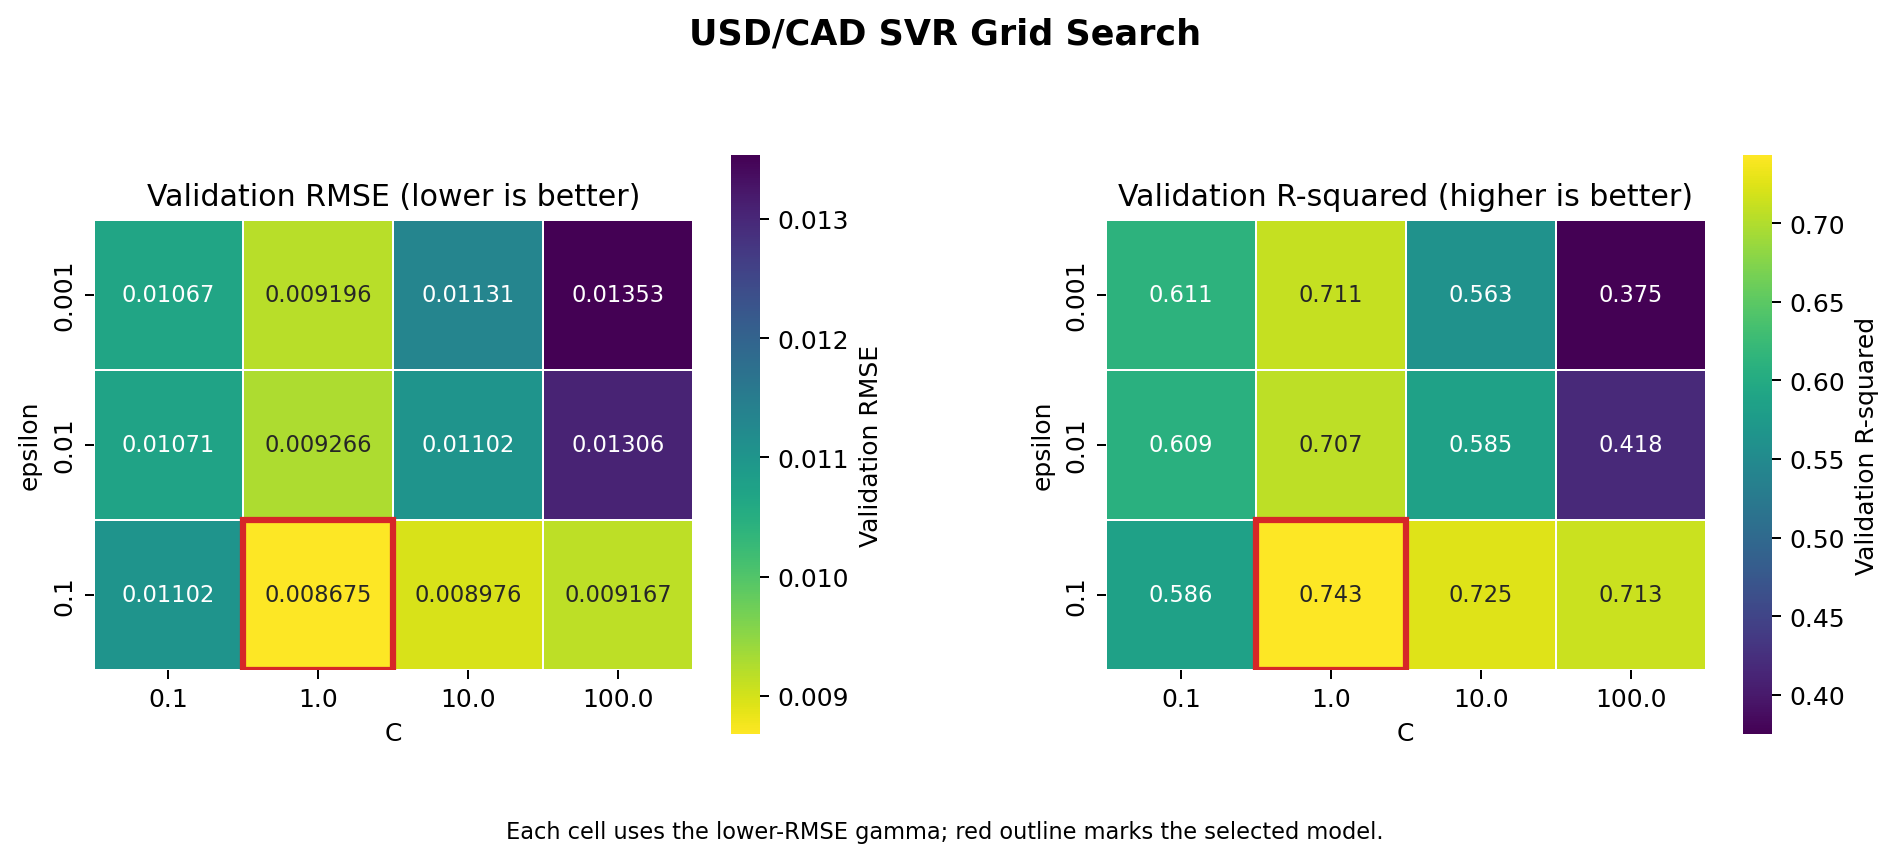
\includegraphics[width=\textwidth]{figures/USD_svr_grid_heatmap.png}
  \caption{USD/CAD SVR grid-search validation metrics.}
  \label{fig:usd_grid}
\end{figure}

\begin{figure}[!t]
  \centering
  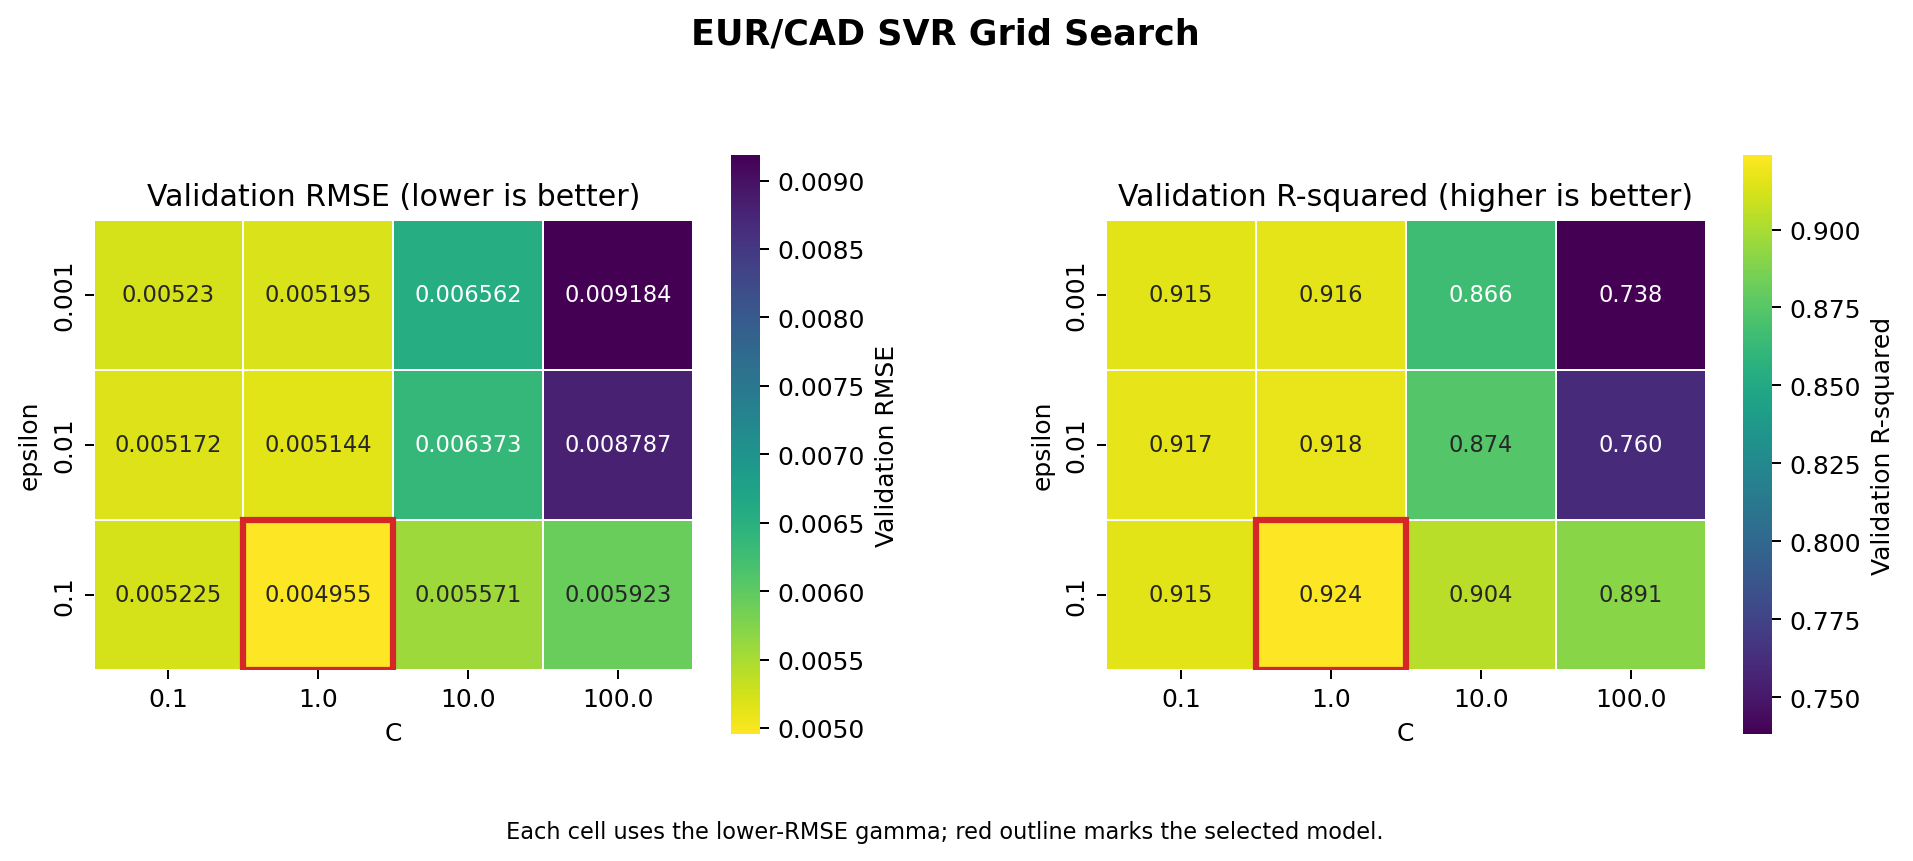
\includegraphics[width=\textwidth]{figures/EUR_svr_grid_heatmap.png}
  \caption{EUR/CAD SVR grid-search validation metrics.}
  \label{fig:eur_grid}
\end{figure}

\begin{figure}[!t]
  \centering
  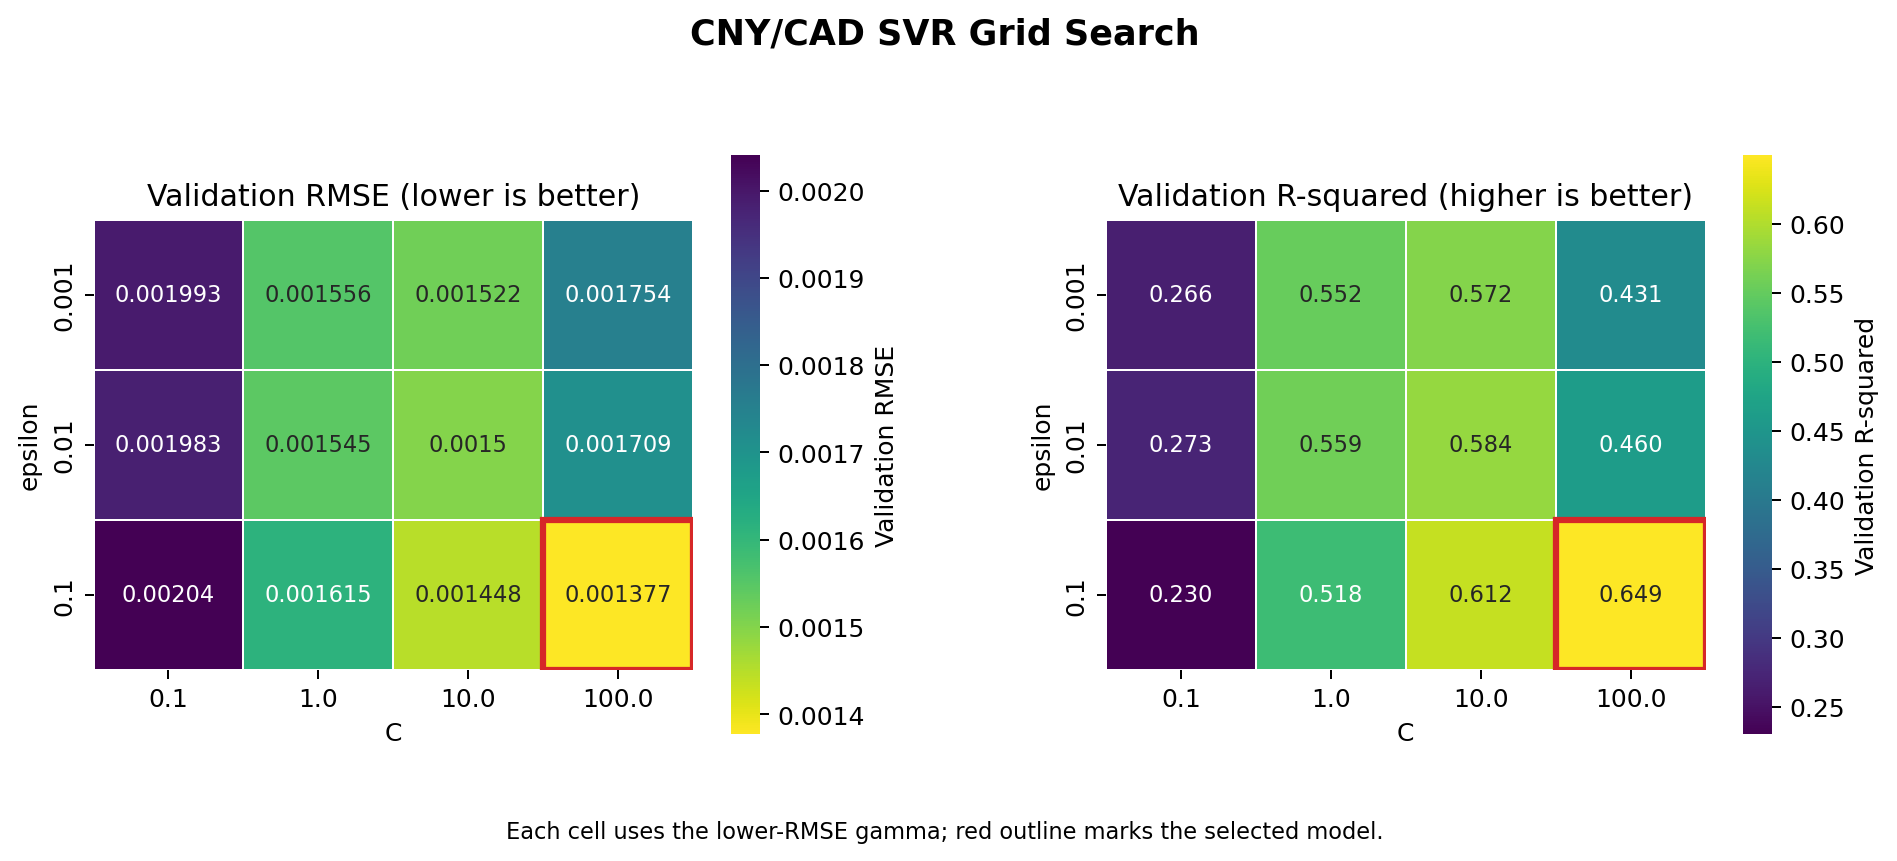
\includegraphics[width=\textwidth]{figures/CNY_svr_grid_heatmap.png}
  \caption{CNY/CAD SVR grid-search validation metrics.}
  \label{fig:cny_grid}
\end{figure}

\subsection{Prediction Plots}

Figure~\ref{fig:predictions} shows actual vs.\ predicted exchange rates on the test set for all three currency pairs.

\begin{figure}[!t]
  \centering
  \begin{subfigure}[b]{\textwidth}
    \centering
    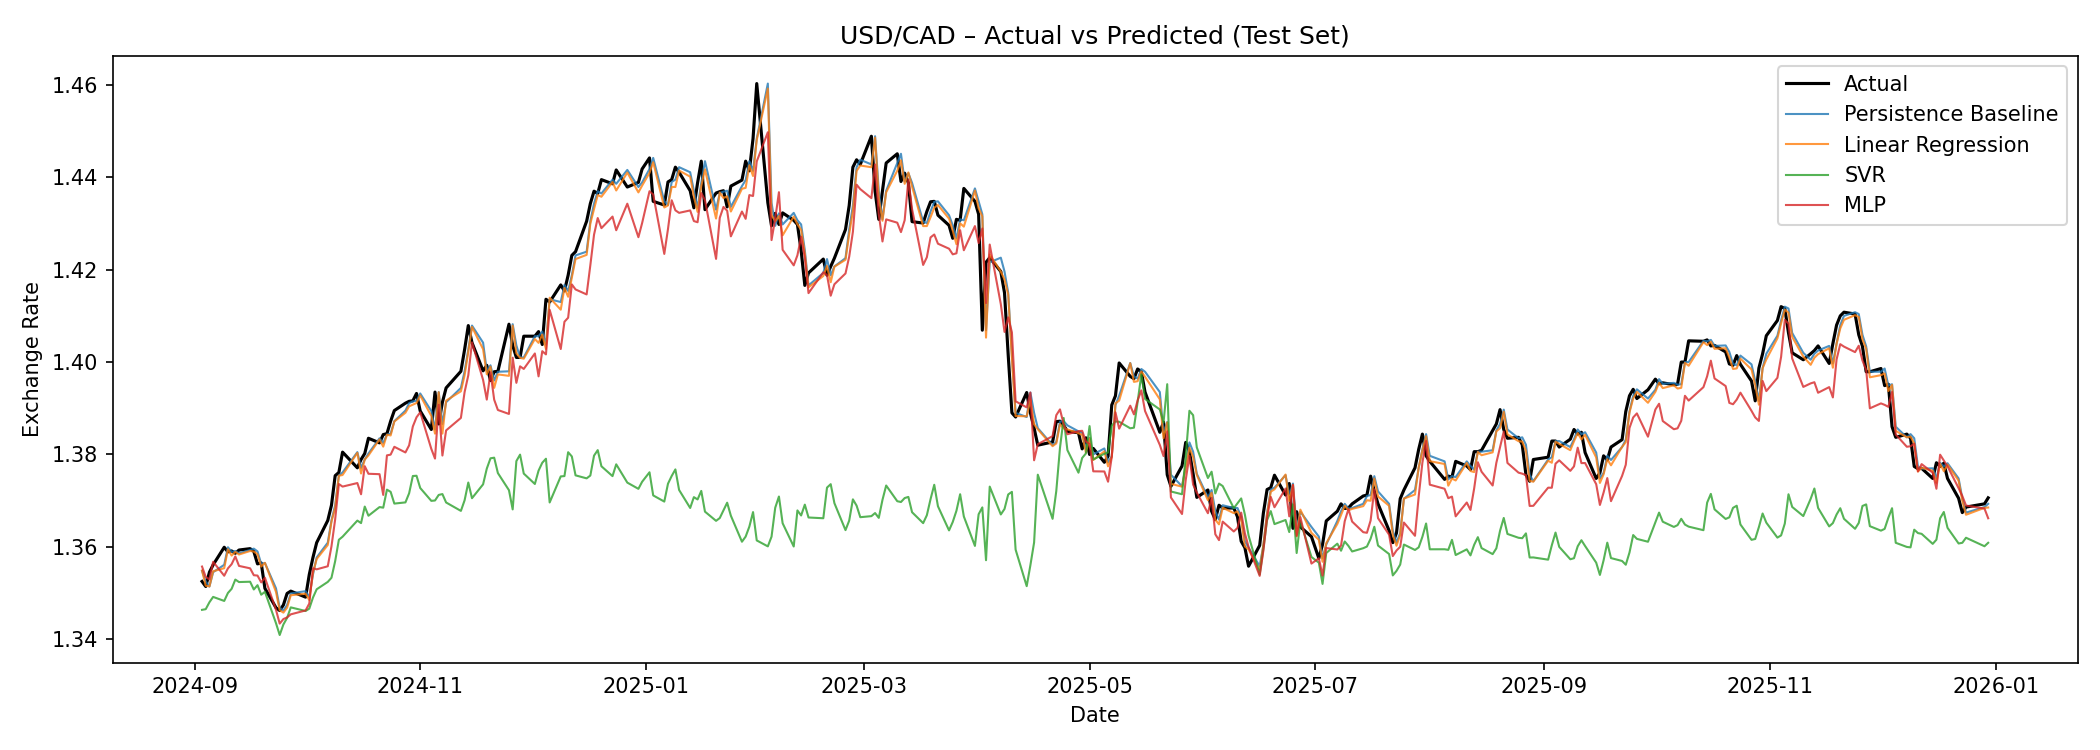
\includegraphics[width=\textwidth]{figures/USD_predictions.png}
    \caption{USD/CAD}
    \label{fig:usd_pred}
  \end{subfigure}\\[4pt]
  \begin{subfigure}[b]{\textwidth}
    \centering
    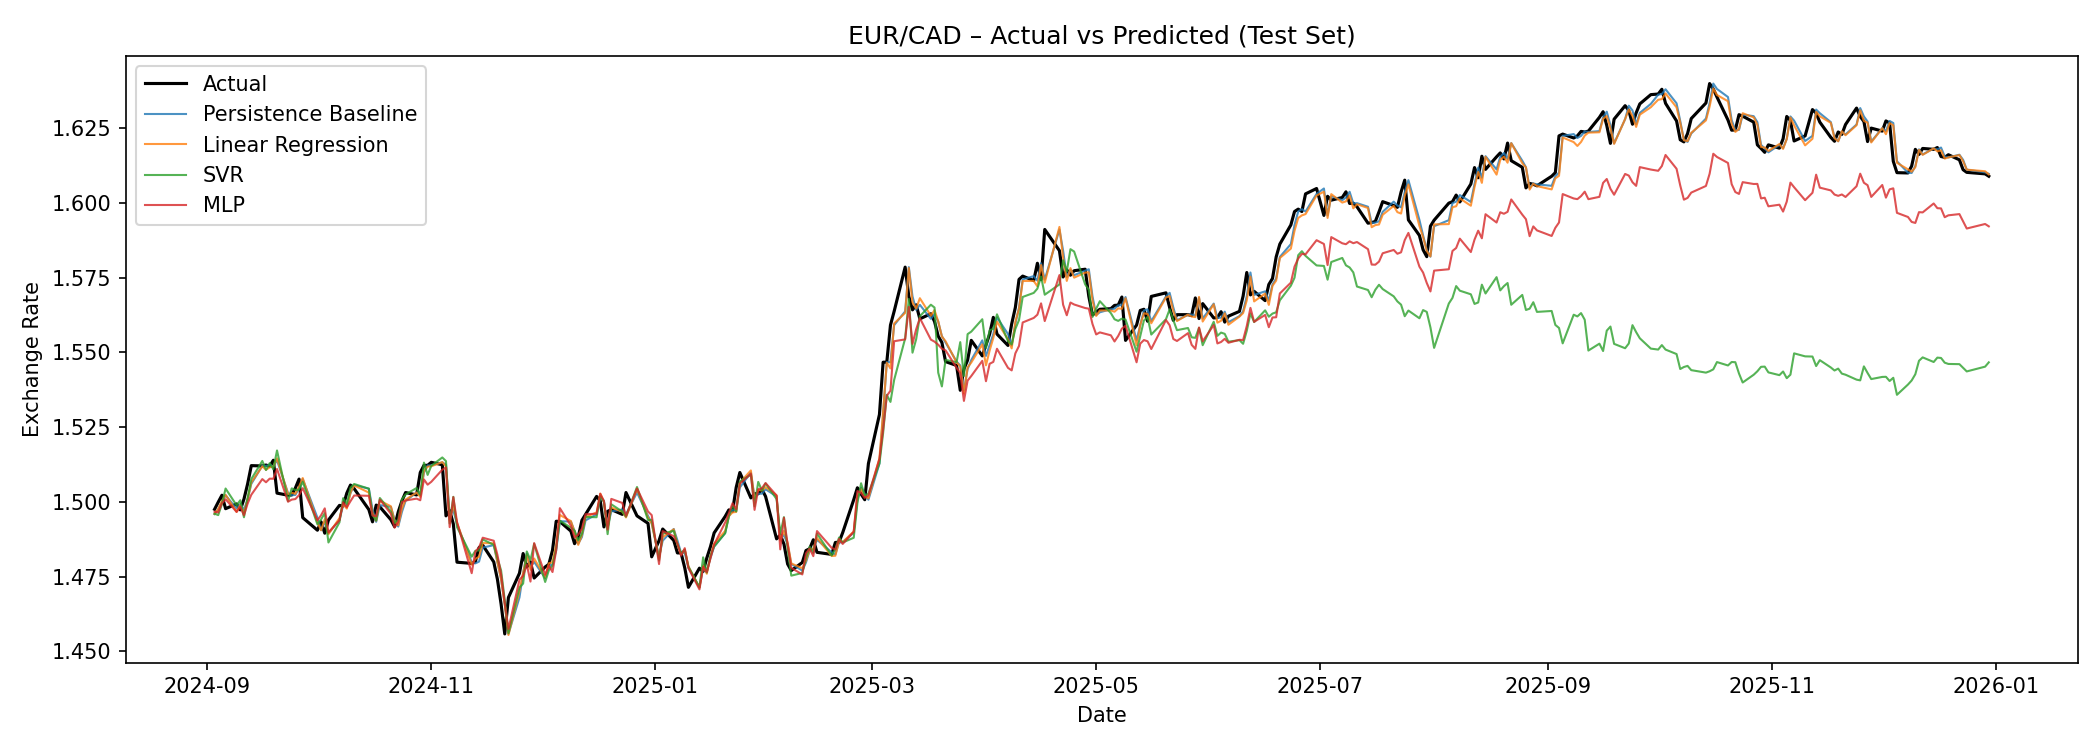
\includegraphics[width=\textwidth]{figures/EUR_predictions.png}
    \caption{EUR/CAD}
    \label{fig:eur_pred}
  \end{subfigure}\\[4pt]
  \begin{subfigure}[b]{\textwidth}
    \centering
    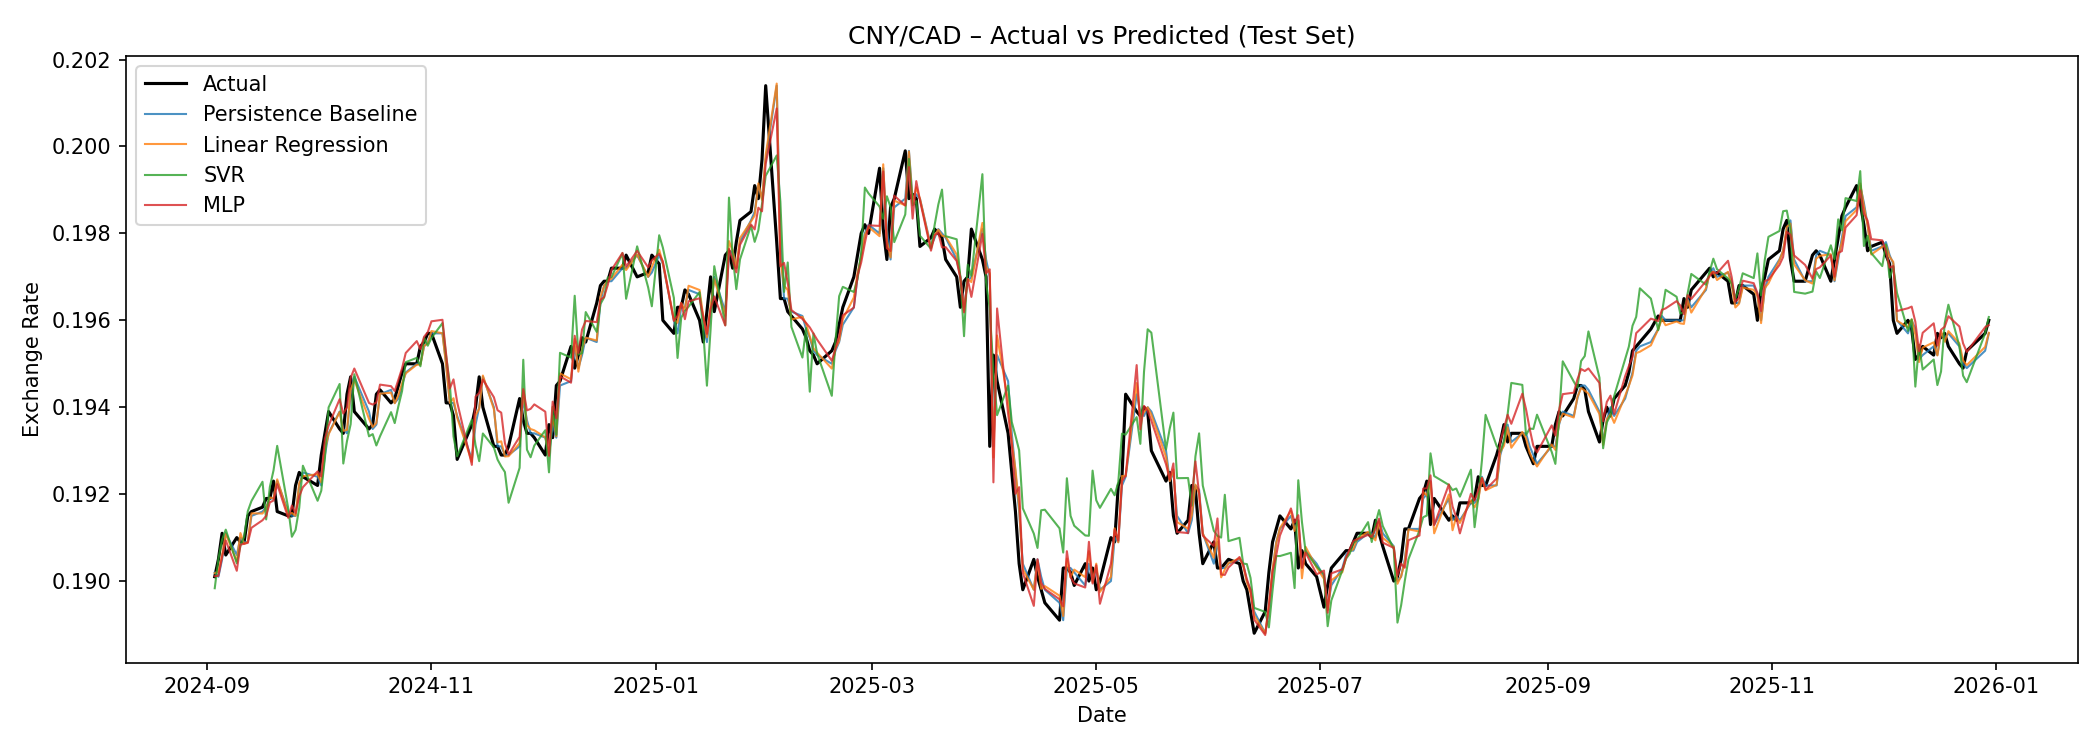
\includegraphics[width=\textwidth]{figures/CNY_predictions.png}
    \caption{CNY/CAD}
    \label{fig:cny_pred}
  \end{subfigure}
  \caption{Actual vs.\ predicted exchange rates on the test set (Persistence, LR, SVR, and MLP). Persistence and Linear Regression track the observed levels closely, while SVR lags substantially on USD/CAD.}
  \label{fig:predictions}
\end{figure}

\subsection{LSTM Predictions}

Figure~\ref{fig:lstm_predictions} shows LSTM predictions on the test set (offset by the 21-day sequence window).

\begin{figure}[!t]
  \centering
  \begin{subfigure}[b]{0.32\textwidth}
    \centering
    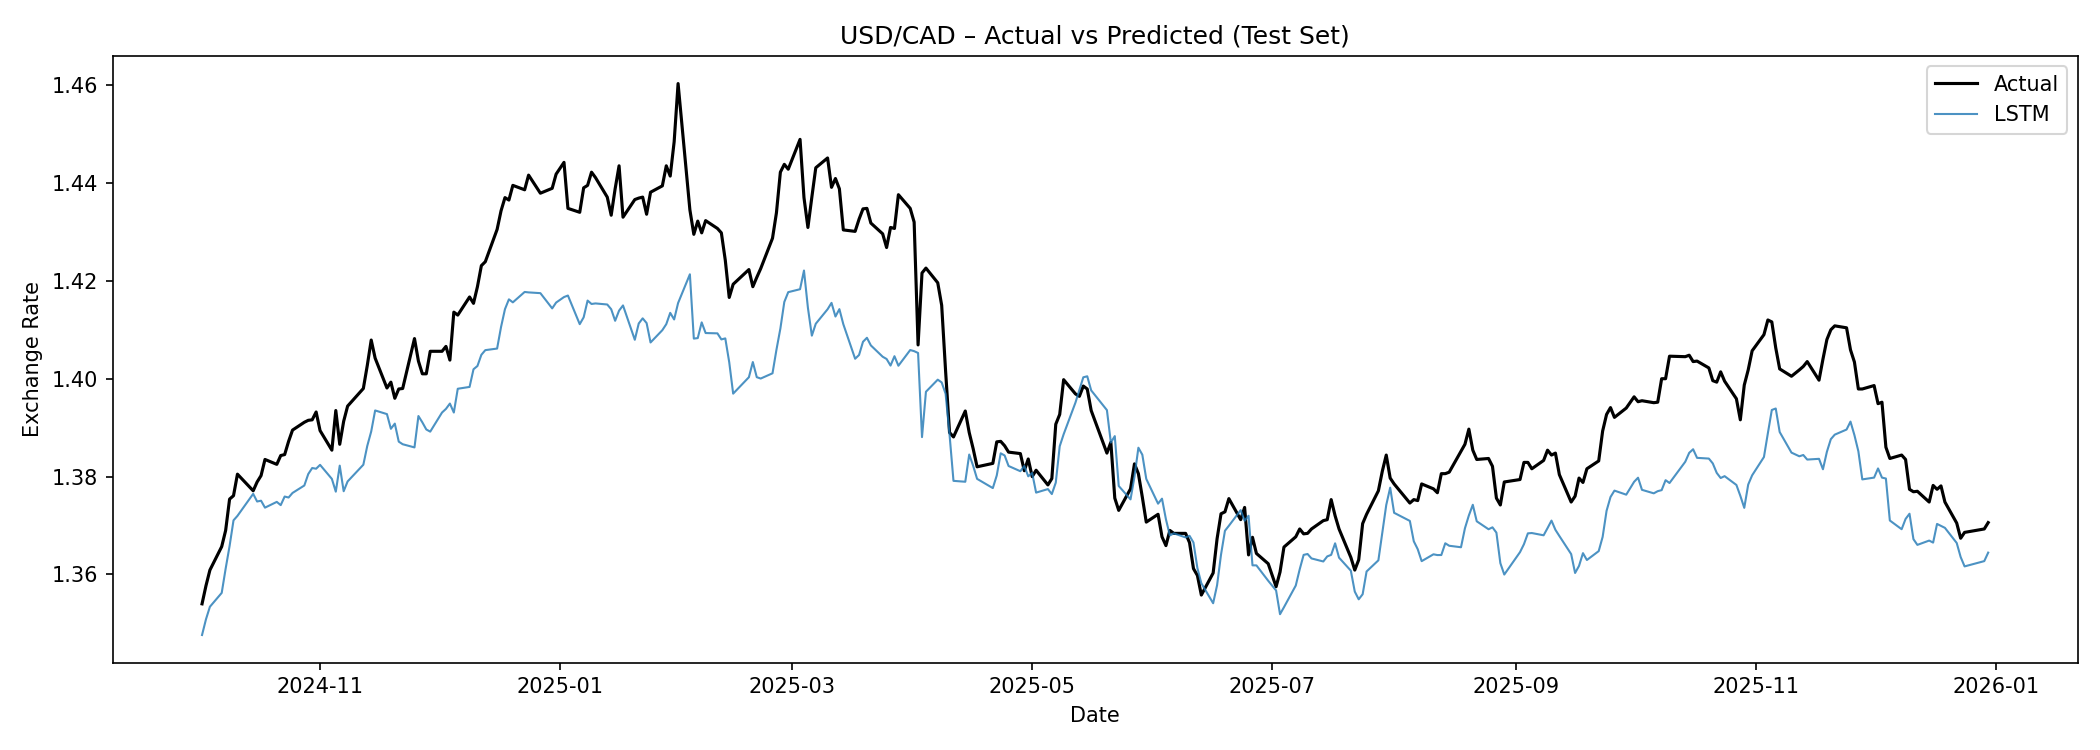
\includegraphics[width=\textwidth]{figures/USD_LSTM_predictions.png}
    \caption{USD/CAD}
  \end{subfigure}\hfill
  \begin{subfigure}[b]{0.32\textwidth}
    \centering
    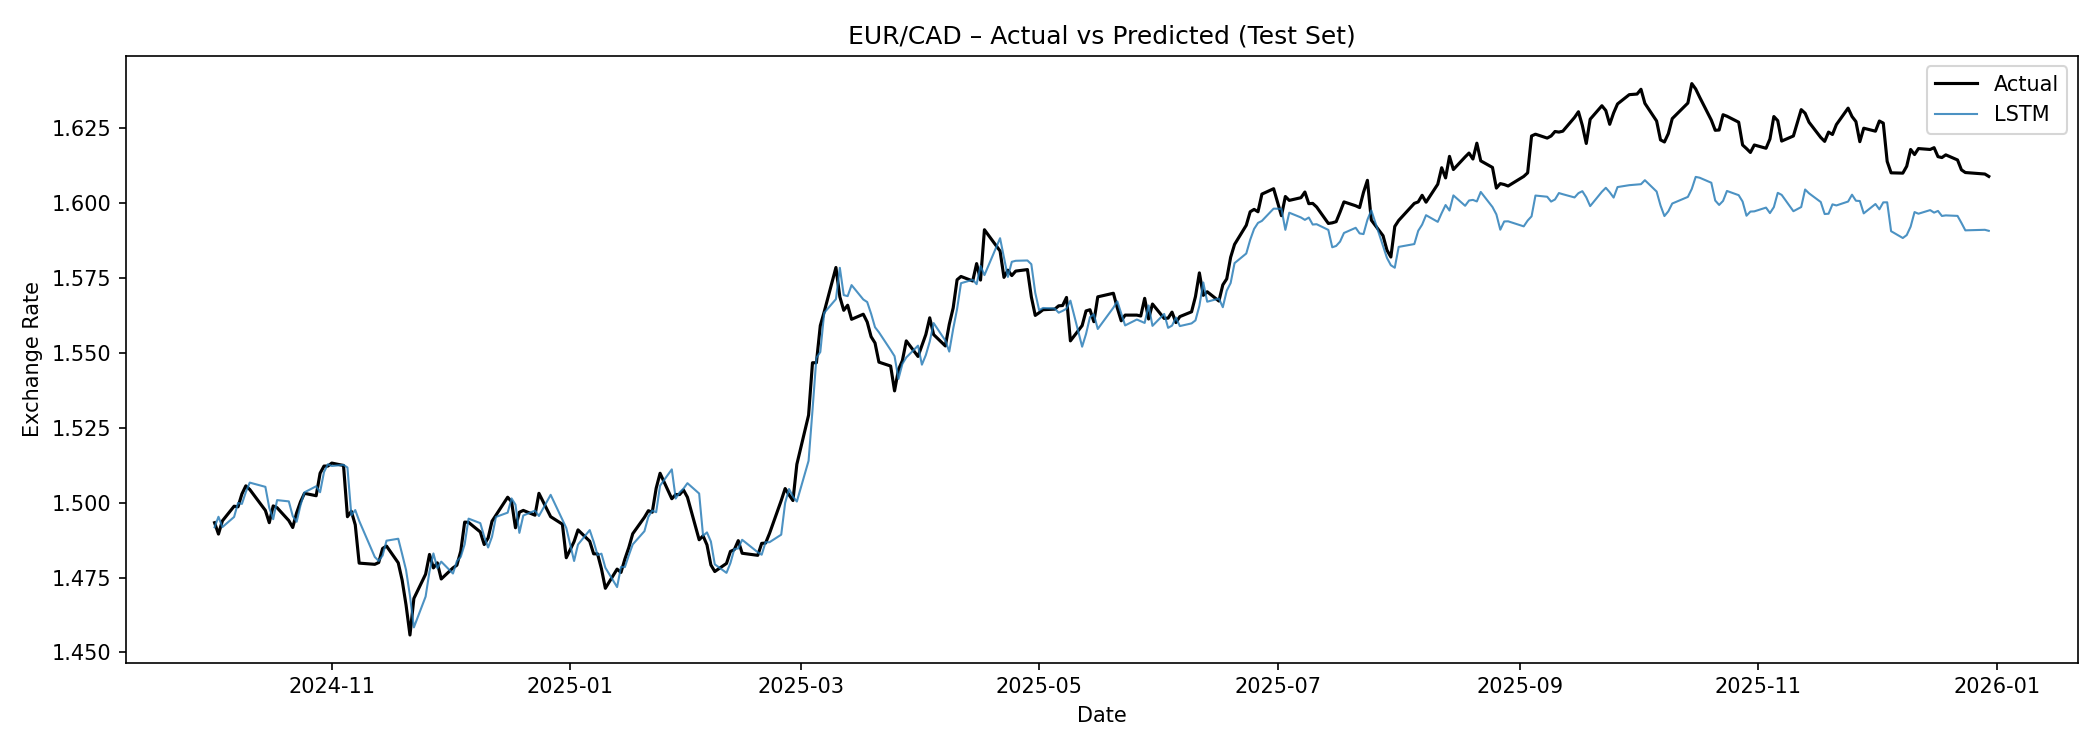
\includegraphics[width=\textwidth]{figures/EUR_LSTM_predictions.png}
    \caption{EUR/CAD}
  \end{subfigure}\hfill
  \begin{subfigure}[b]{0.32\textwidth}
    \centering
    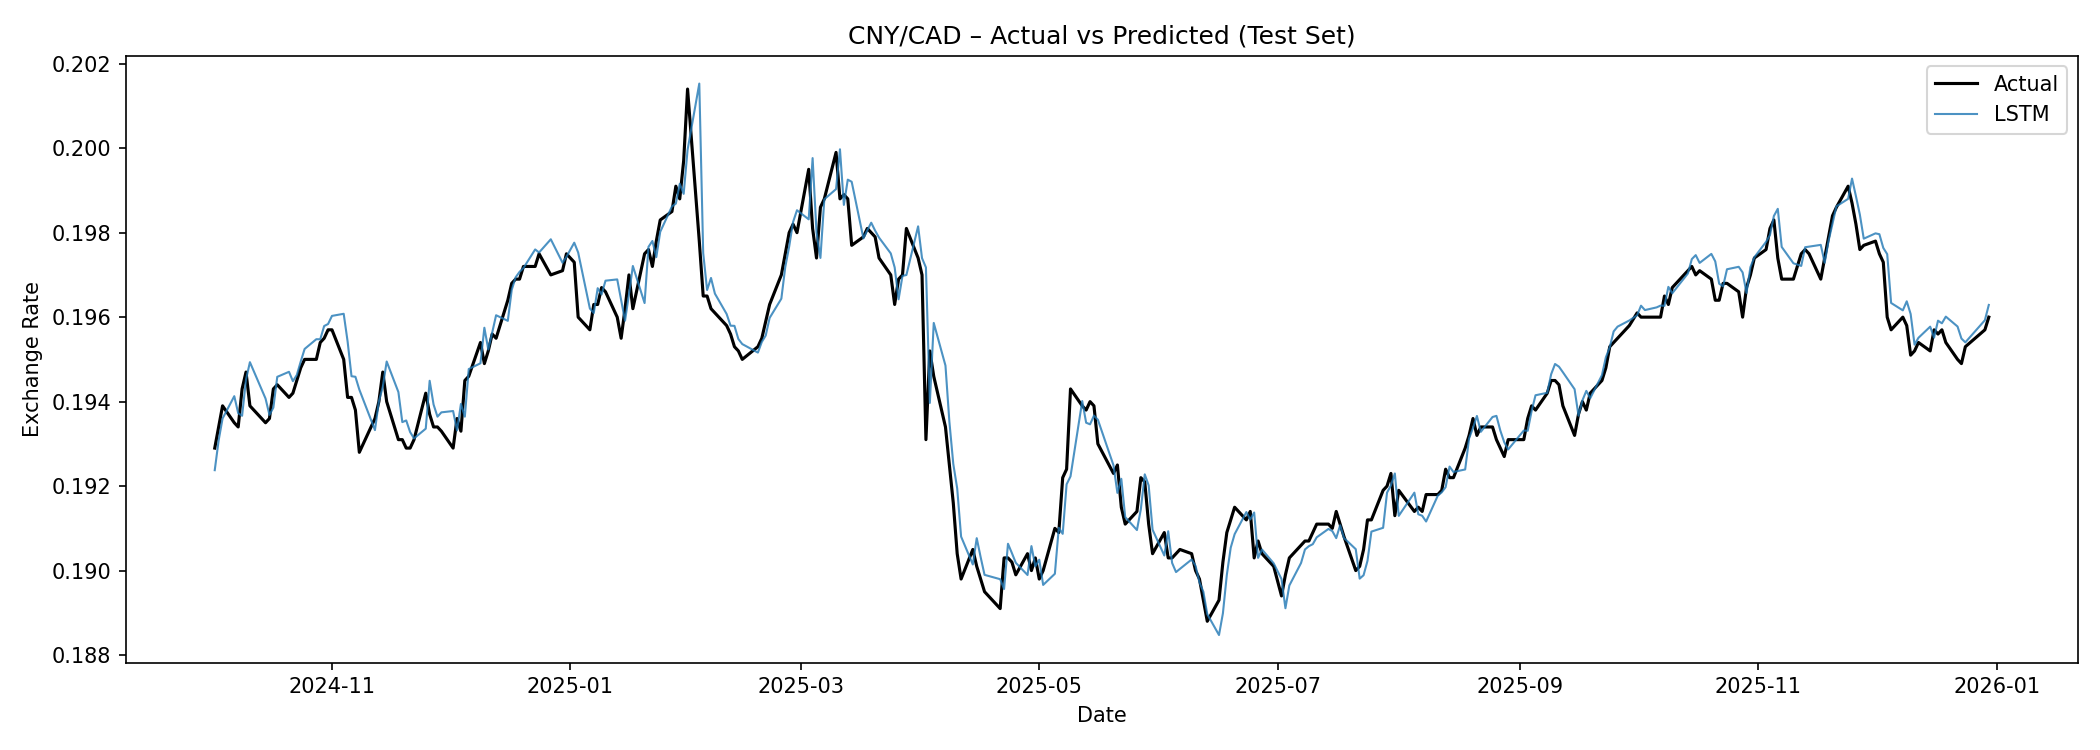
\includegraphics[width=\textwidth]{figures/CNY_LSTM_predictions.png}
    \caption{CNY/CAD}
  \end{subfigure}
  \caption{LSTM predictions vs.\ actual exchange rates on the test set. The LSTM closely tracks EUR/CAD and CNY/CAD ($R^2 > 0.93$) but shows more deviation on USD/CAD.}
  \label{fig:lstm_predictions}
\end{figure}

\section{Discussion}

\subsection{Persistence Baseline Is Strongest}

The persistence forecast achieves the lowest RMSE on all three pairs: 0.0044 for USD/CAD, 0.0052 for EUR/CAD, and 0.0006 for CNY/CAD. Linear regression is close but does not improve on persistence. Consequently, the high $R^2$ values primarily reflect strong level autocorrelation rather than evidence that the learned models extract incremental predictive information. This comparison is essential for exchange-rate forecasting, where random-walk-style baselines are historically difficult to beat~[2].

\subsection{Impact of Target Normalization}

In our initial experiments, SVR and MLP produced negative $R^2$ values due to a feature--target scale mismatch: features were standardized while targets remained in their original scale. After normalizing targets with a separate \texttt{StandardScaler}, MLP performance improved dramatically (e.g., USD/CAD $R^2$ from $-4.87$ to $0.92$). This underscores the importance of consistent preprocessing for gradient-based and kernel-based methods. Linear regression, being scale-invariant, was unaffected.

\subsection{MLP and LSTM Performance}

With target normalization, both the MLP and LSTM achieve strong results on EUR/CAD ($R^2 \approx 0.935$) and CNY/CAD ($R^2 \approx 0.94$). The LSTM slightly outperforms the MLP on EUR/CAD ($R^2 = 0.936$ vs.\ $0.935$), suggesting that its ability to model temporal dependencies provides a modest advantage for more volatile pairs. However, on USD/CAD the LSTM lags behind ($R^2 = 0.54$), likely because the shorter effective test set (reduced by the 21-day sequence window) makes evaluation noisier.

\section{Conclusions}

The persistence forecast achieves the best test performance on all three currency pairs, narrowly outperforming linear regression. This result shows that strong $R^2$ values for exchange-rate levels do not by themselves establish value beyond a random-walk forecast. After correcting a feature--target scale mismatch via target normalization, MLP and LSTM are competitive on EUR/CAD and CNY/CAD but still trail persistence. SVR benefits from grid-searched hyperparameters yet remains limited by the $\varepsilon$-insensitive formulation on near-random-walk data, particularly for USD/CAD.

\textbf{Future work:} (a)~implement expanding- or rolling-window walk-forward validation, (b)~predict returns or direction rather than only levels, (c)~add exogenous features such as interest rates, commodity prices, and VIX, and (d)~evaluate longer horizons and Transformer-based architectures.


\section*{References}

\medskip
{
\small

[1] Meese, R.A.\ \& Rogoff, K.\ (1983) Empirical exchange rate models of the seventies: Do they fit out of sample? {\it Journal of International Economics} {\bf 14}(1--2):3--24.

[2] Rossi, B.\ (2013) Exchange rate predictability. {\it Journal of Economic Literature} {\bf 51}(4):1063--1119.

[3] Vapnik, V.N.\ (1995) {\it The Nature of Statistical Learning Theory.} New York: Springer-Verlag.

[4] Hornik, K., Stinchcombe, M.\ \& White, H.\ (1989) Multilayer feedforward networks are universal approximators. {\it Neural Networks} {\bf 2}(5):359--366.

[5] Pedregosa, F.\ et al.\ (2011) Scikit-learn: Machine learning in Python. {\it Journal of Machine Learning Research} {\bf 12}:2825--2830.

[6] Smola, A.J.\ \& Sch\"olkopf, B.\ (2004) A tutorial on support vector regression. {\it Statistics and Computing} {\bf 14}(3):199--222.

[7] Paszke, A.\ et al.\ (2019) PyTorch: An imperative style, high-performance deep learning library. In {\it Advances in Neural Information Processing Systems 32}, pp.\ 8026--8037.

[8] Kingma, D.P.\ \& Ba, J.\ (2015) Adam: A method for stochastic optimization. In {\it Proc.\ 3rd International Conference on Learning Representations (ICLR)}.

[9] Bank of Canada (2025) Valet API documentation.~\url{https://www.bankofcanada.ca/valet/docs}.

[10] Hochreiter, S.\ \& Schmidhuber, J.\ (1997) Long short-term memory. {\it Neural Computation} {\bf 9}(8):1735--1780.
}

\section*{Appendix}

\subsection*{A. Hyperparameters}

\begin{table}[h]
  \caption{Hyperparameters for SVR and MLP models.}
  \label{tab:hyperparams}
  \centering
  \begin{tabular}{lll}
    \toprule
    Model & Parameter & Value \\
    \midrule
    SVR & Kernel & RBF \\
    SVR & $C$ (grid) & \{0.1, 1.0, 10.0, 100.0\} \\
    SVR & $\varepsilon$ (grid) & \{0.001, 0.01, 0.1\} \\
    SVR & $\gamma$ (grid) & \{scale, auto\} \\
    \midrule
    MLP & Hidden layers & [128, 64, 32] \\
    MLP & Activation & ReLU \\
    MLP & Dropout rate & 0.2 \\
    MLP & Batch normalization & Yes \\
    MLP & Optimizer & Adam \\
    MLP & Learning rate & $10^{-3}$ \\
    MLP & Weight decay & $10^{-5}$ \\
    MLP & Batch size & 64 \\
    MLP & Max epochs & 200 \\
    MLP & Early stopping patience & 20 \\
    MLP & LR scheduler & ReduceLROnPlateau (factor=0.5, patience=10) \\
    \midrule
    LSTM & Hidden size & 64 \\
    LSTM & Number of layers & 2 \\
    LSTM & Dropout rate & 0.2 \\
    LSTM & Sequence length & 21 \\
    LSTM & Optimizer & Adam \\
    LSTM & Learning rate & $10^{-3}$ \\
    LSTM & Weight decay & $10^{-5}$ \\
    LSTM & Batch size & 64 \\
    LSTM & Max epochs & 200 \\
    LSTM & Early stopping patience & 20 \\
    LSTM & LR scheduler & ReduceLROnPlateau (factor=0.5, patience=10) \\
    \bottomrule
  \end{tabular}
\end{table}

\subsection*{B. Residual Histograms}

Figure~\ref{fig:residuals} shows residual distributions for all learned-model--currency combinations. Linear Regression and MLP residuals are tightly centered around zero, while SVR exhibits wider distributions on some pairs. LSTM residuals are comparable to MLP on EUR and CNY.

\begin{figure}[h]
  \centering
  \begin{subfigure}[b]{0.24\textwidth}
    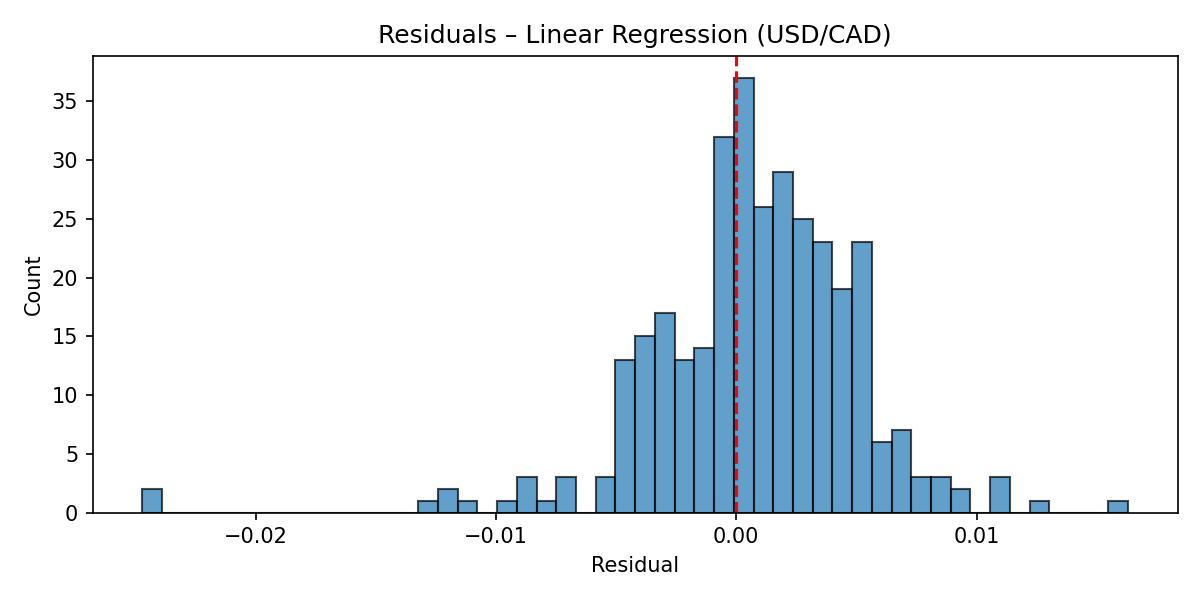
\includegraphics[width=\textwidth]{figures/USD_Linear_Regression_residuals.png}
    \caption{LR -- USD}
  \end{subfigure}\hfill
  \begin{subfigure}[b]{0.24\textwidth}
    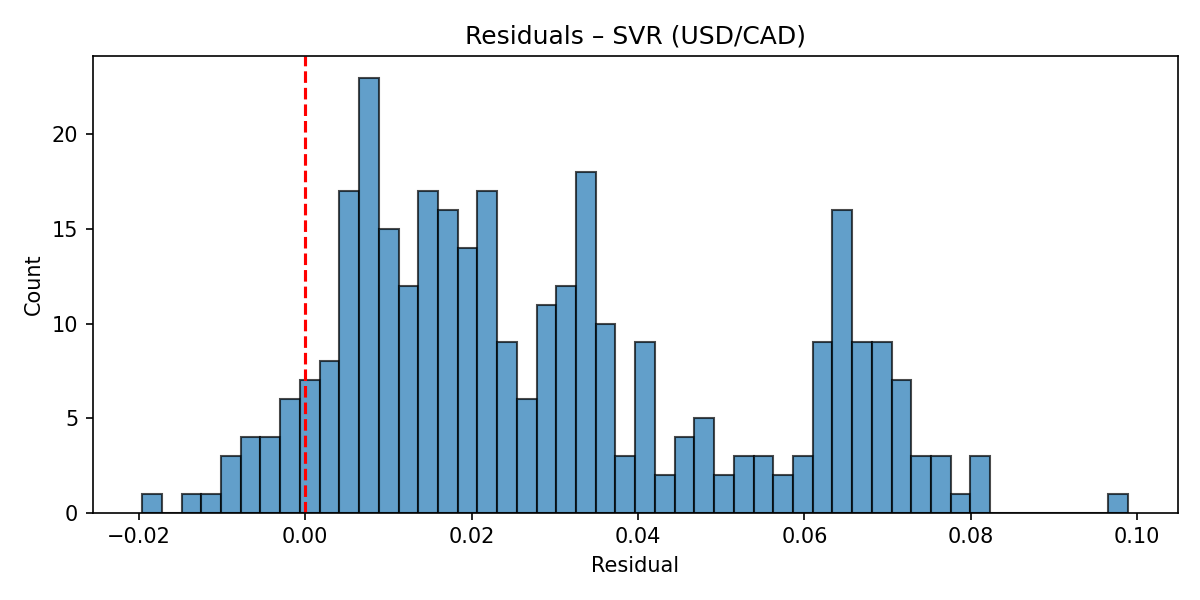
\includegraphics[width=\textwidth]{figures/USD_SVR_residuals.png}
    \caption{SVR -- USD}
  \end{subfigure}\hfill
  \begin{subfigure}[b]{0.24\textwidth}
    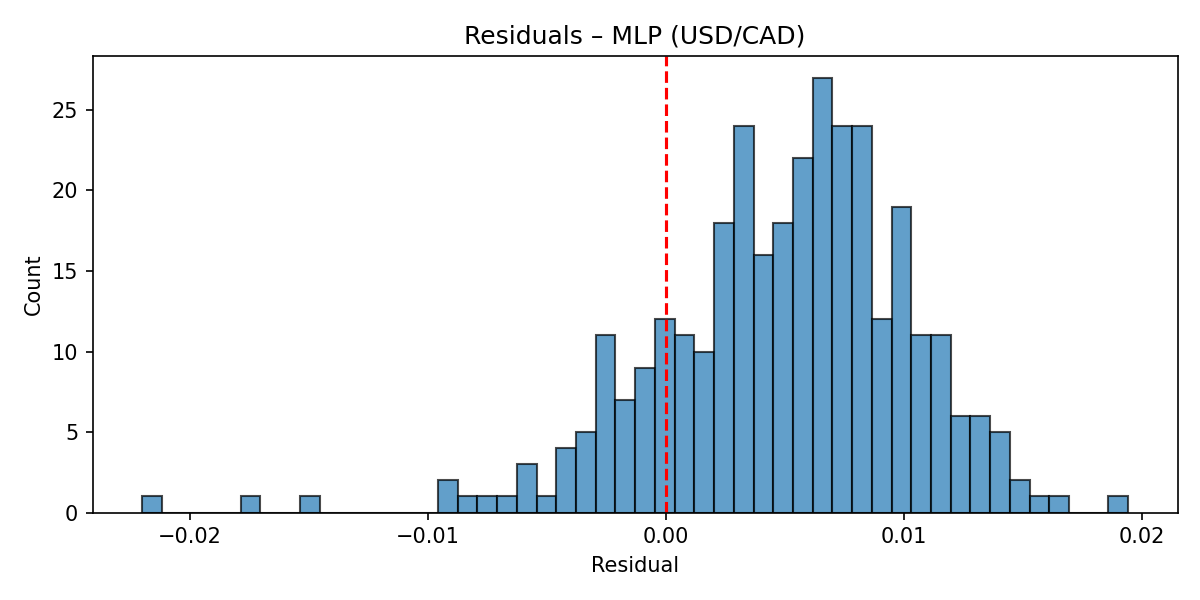
\includegraphics[width=\textwidth]{figures/USD_MLP_residuals.png}
    \caption{MLP -- USD}
  \end{subfigure}\hfill
  \begin{subfigure}[b]{0.24\textwidth}
    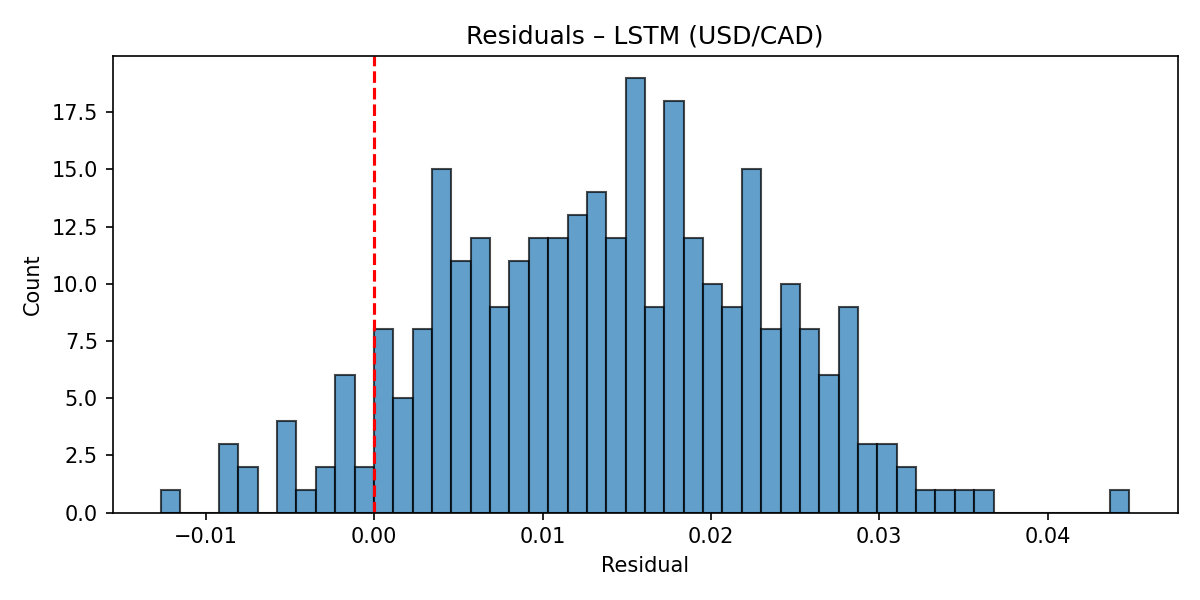
\includegraphics[width=\textwidth]{figures/USD_LSTM_residuals.png}
    \caption{LSTM -- USD}
  \end{subfigure}\\[4pt]
  \begin{subfigure}[b]{0.24\textwidth}
    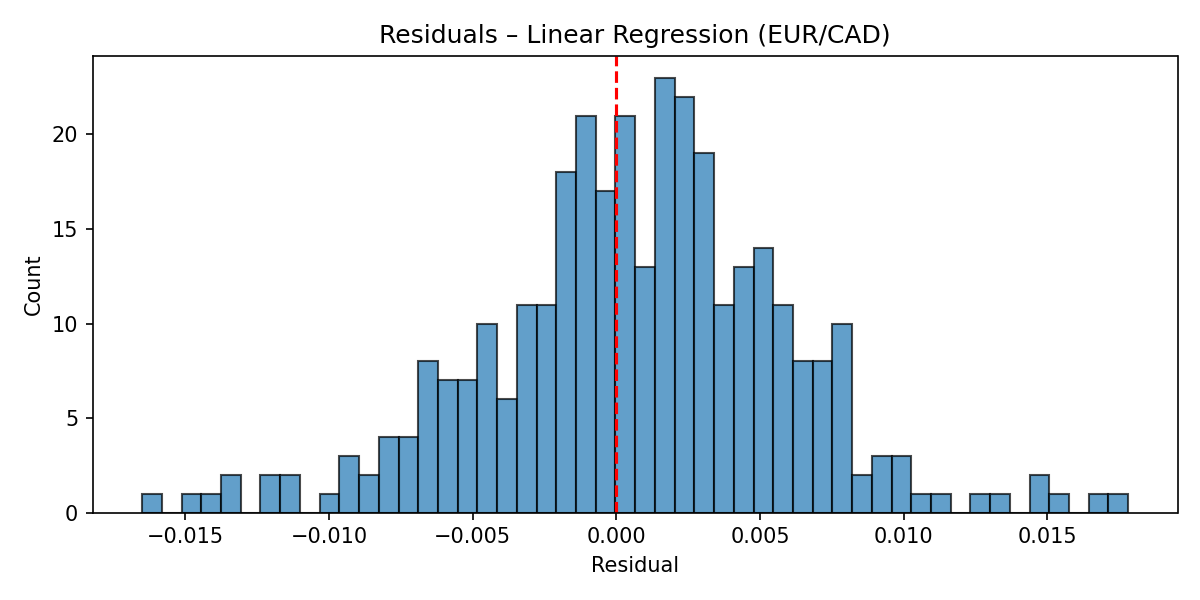
\includegraphics[width=\textwidth]{figures/EUR_Linear_Regression_residuals.png}
    \caption{LR -- EUR}
  \end{subfigure}\hfill
  \begin{subfigure}[b]{0.24\textwidth}
    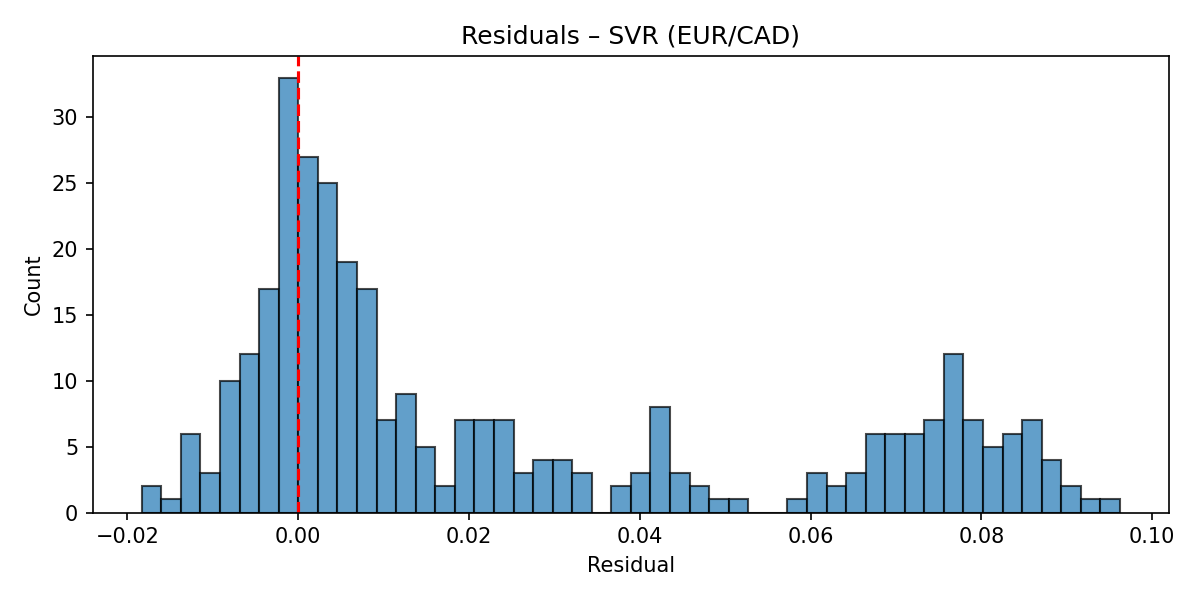
\includegraphics[width=\textwidth]{figures/EUR_SVR_residuals.png}
    \caption{SVR -- EUR}
  \end{subfigure}\hfill
  \begin{subfigure}[b]{0.24\textwidth}
    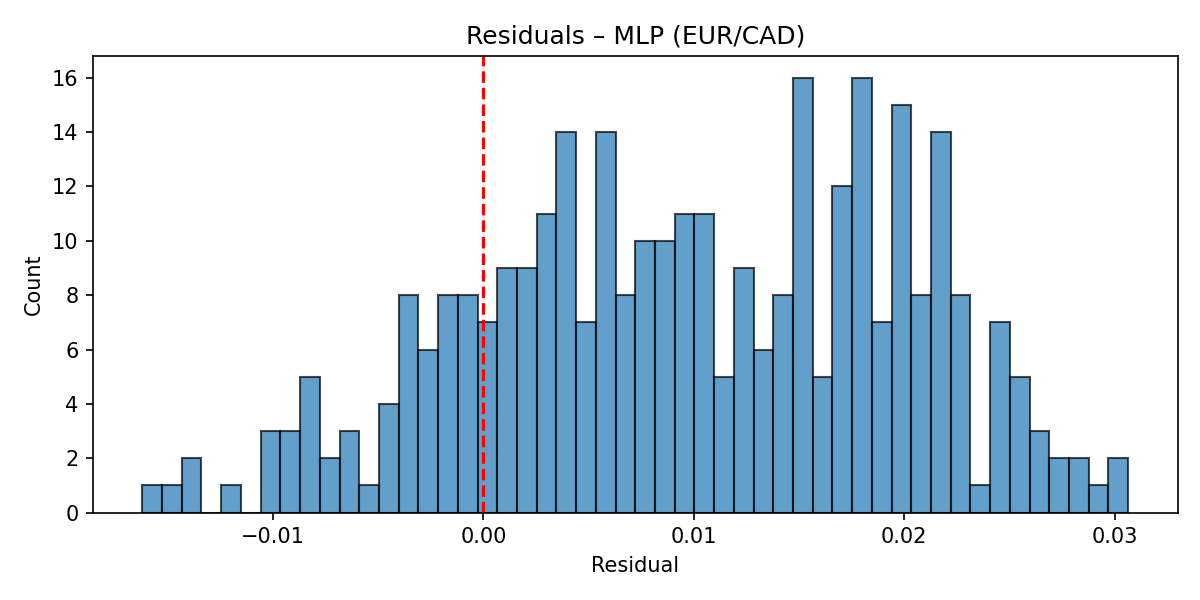
\includegraphics[width=\textwidth]{figures/EUR_MLP_residuals.png}
    \caption{MLP -- EUR}
  \end{subfigure}\hfill
  \begin{subfigure}[b]{0.24\textwidth}
    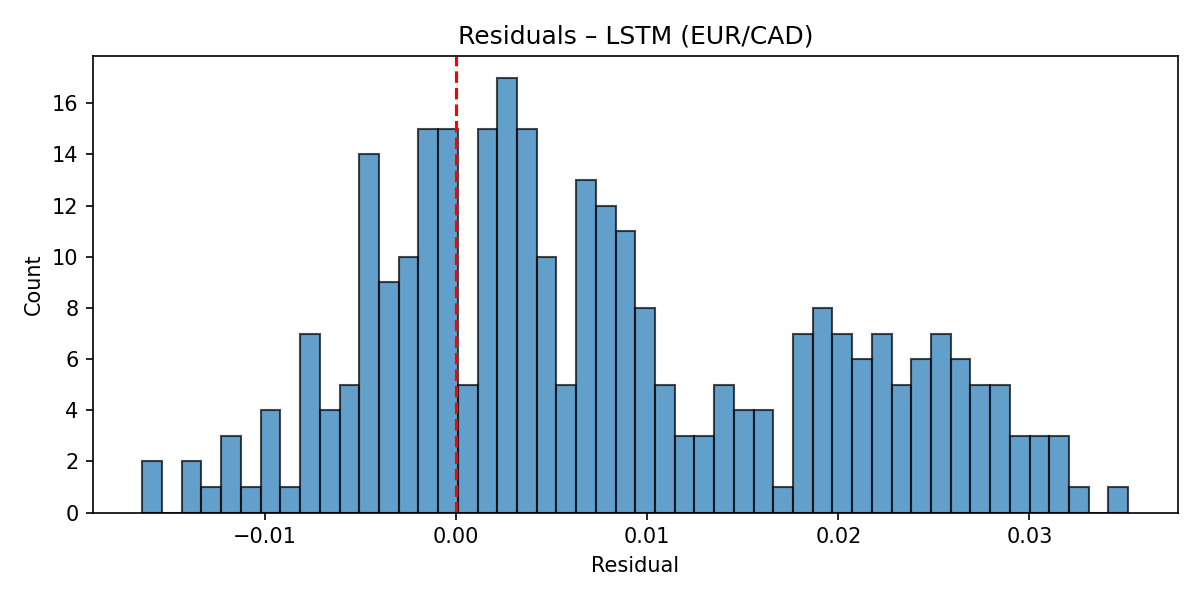
\includegraphics[width=\textwidth]{figures/EUR_LSTM_residuals.png}
    \caption{LSTM -- EUR}
  \end{subfigure}\\[4pt]
  \begin{subfigure}[b]{0.24\textwidth}
    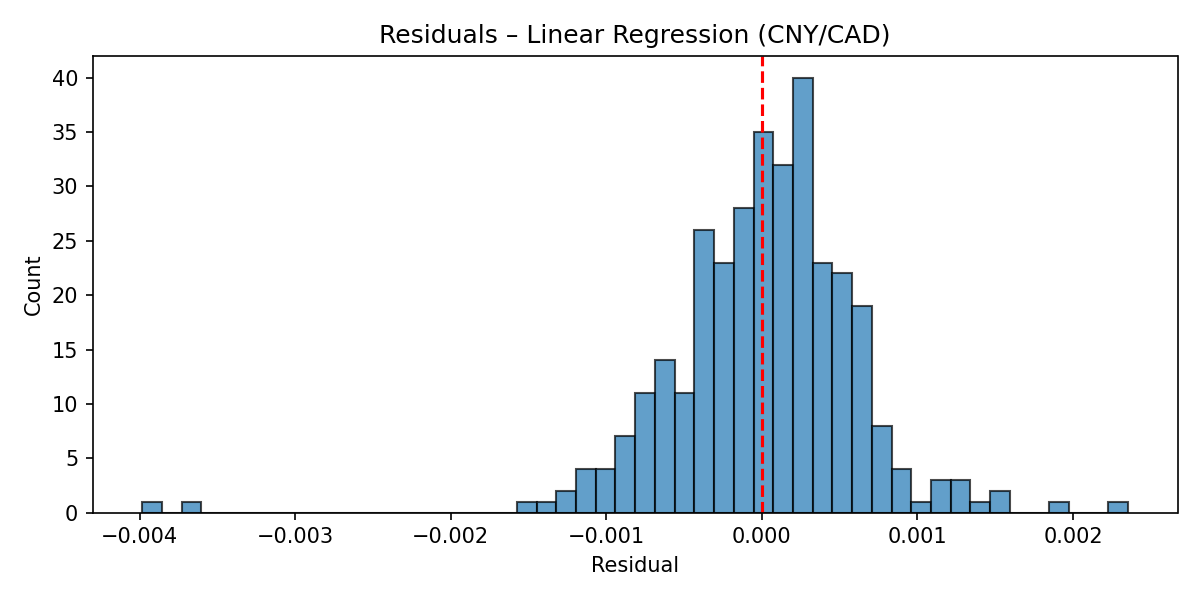
\includegraphics[width=\textwidth]{figures/CNY_Linear_Regression_residuals.png}
    \caption{LR -- CNY}
  \end{subfigure}\hfill
  \begin{subfigure}[b]{0.24\textwidth}
    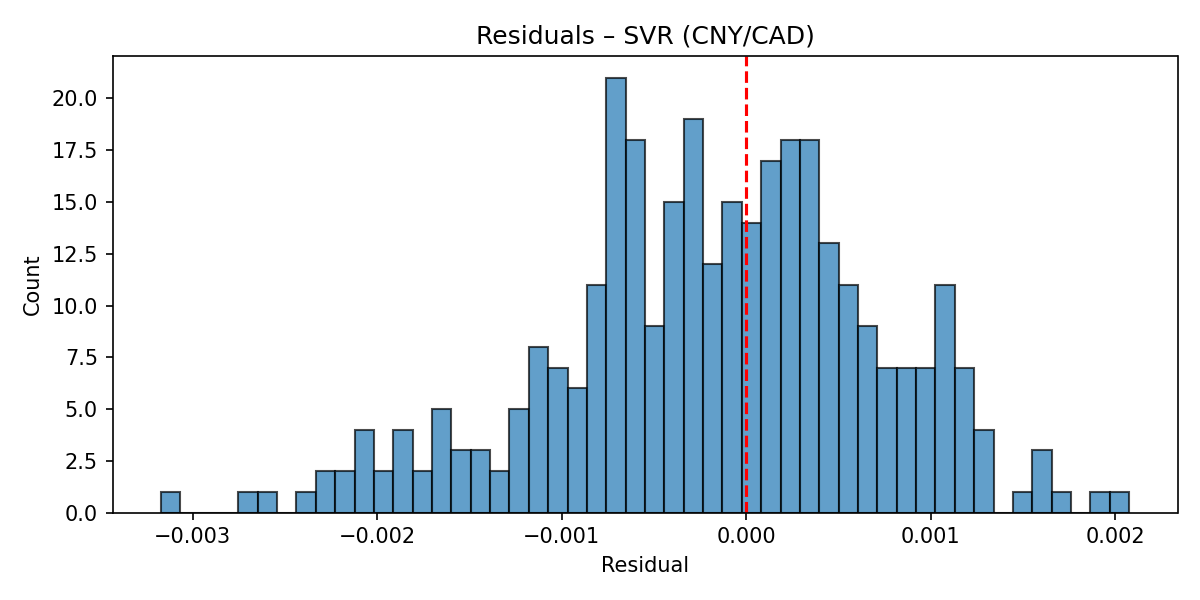
\includegraphics[width=\textwidth]{figures/CNY_SVR_residuals.png}
    \caption{SVR -- CNY}
  \end{subfigure}\hfill
  \begin{subfigure}[b]{0.24\textwidth}
    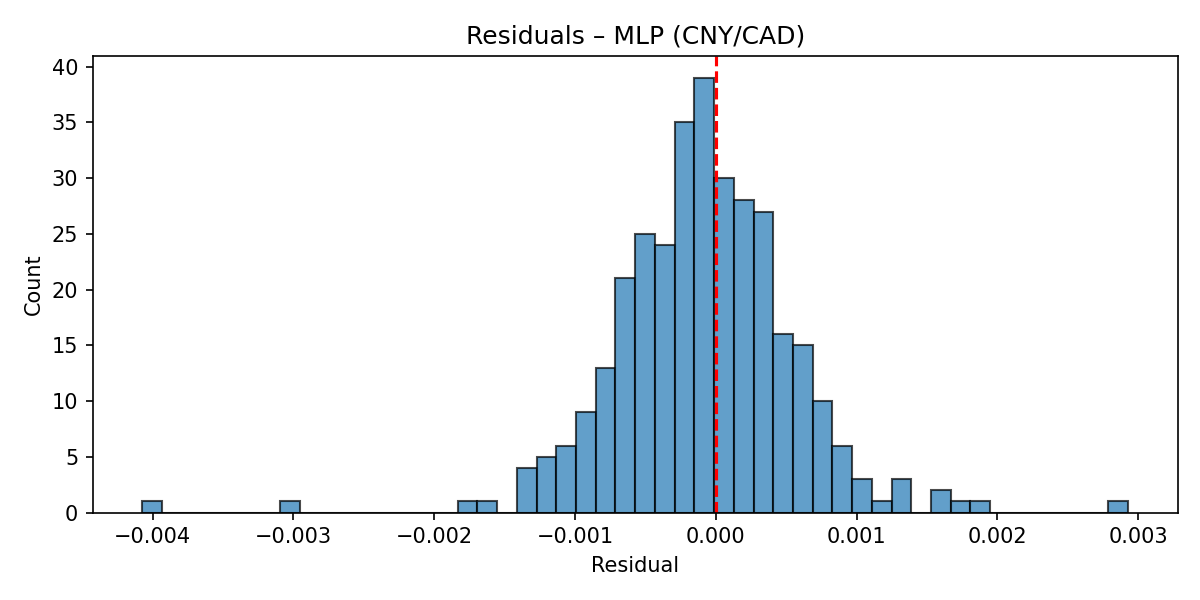
\includegraphics[width=\textwidth]{figures/CNY_MLP_residuals.png}
    \caption{MLP -- CNY}
  \end{subfigure}\hfill
  \begin{subfigure}[b]{0.24\textwidth}
    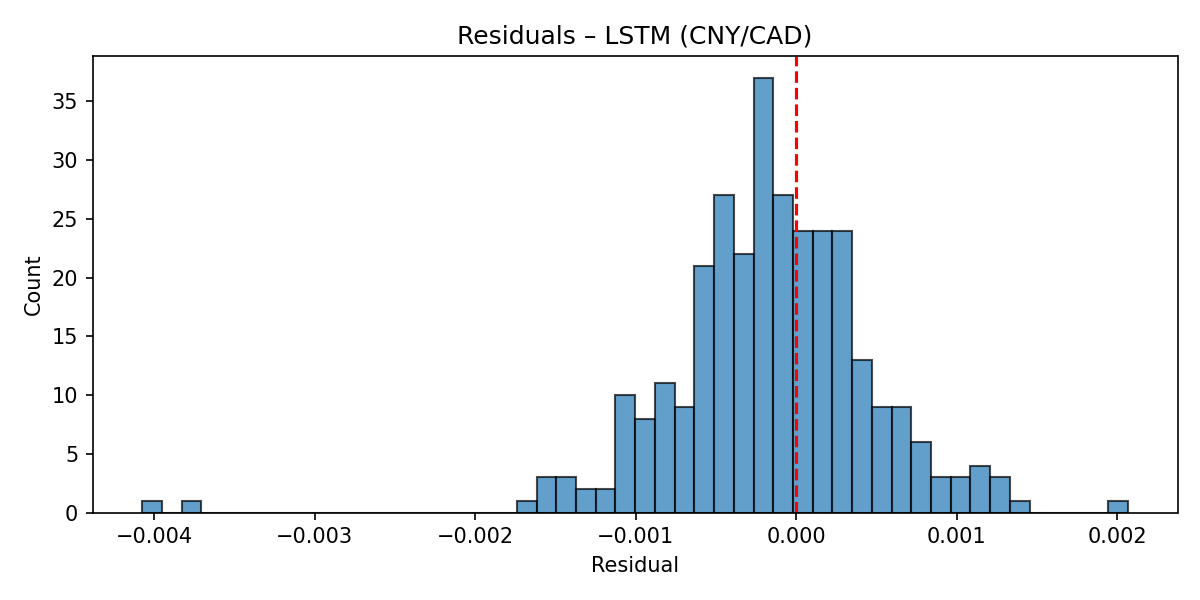
\includegraphics[width=\textwidth]{figures/CNY_LSTM_residuals.png}
    \caption{LSTM -- CNY}
  \end{subfigure}
  \caption{Residual histograms for all learned-model--currency pair combinations. The red dashed line marks zero residual.}
  \label{fig:residuals}
\end{figure}

\subsection*{C. Source Code}

The code is organized as: \texttt{main.py} (entry point), \texttt{config.py} (hyperparameters and tuning grids), \texttt{src/data\_loader.py} (data download), \texttt{src/preprocessing.py} (features, splitting, and target scaling), \texttt{src/models.py} (model definitions including LSTM), \texttt{src/train.py} (training, SVR grid search, LSTM training), \texttt{src/evaluate.py} (evaluation), \texttt{src/utils.py} (utilities). All figures are generated by running \texttt{python main.py}. Data from the Bank of Canada Valet API~[9] (public, no key required).

\subsection*{D. Presentation Follow-Up Questions}

\textbf{SVR penalty ($C$).} The parameter $C$ controls the trade-off between model flatness and tolerance for training errors. Large $C$ fits training data more tightly but risks overfitting; small $C$ produces a smoother function. Our grid search over $C \in \{0.1, 1, 10, 100\}$ selects the best value per pair, but even optimal $C$ yields negative $R^2$ on USD/CAD because the $\varepsilon$-insensitive tube collapses predictions toward the mean on highly autocorrelated series.

\textbf{Batch size selection.} We use mini-batches of 64 rather than a single full batch. Mini-batches introduce gradient noise that acts as implicit regularization, helping escape sharp local minima. Full-batch training computes exact gradients but tends to converge to solutions that generalize poorly. The size 64 balances computational efficiency with sufficient noise for regularization.

\textbf{LSTM depth.} We use 2 stacked LSTM layers: the first captures low-level temporal patterns, the second learns higher-order dependencies over those representations. A single layer may underfit complex dynamics, while 3+ layers risk overfitting given our modest training set (~1,535 samples). Dropout (0.2) between layers further mitigates overfitting.


\section*{AI Usage}

We used AI tools for brainstorming, debugging, and sanity-checking our work. Specifically, AI assisted with debugging the feature--target scale mismatch in preprocessing, researching best practices for LSTM sliding-window construction, and verifying early stopping logic. All model design decisions, experimental methodology, feature engineering choices, and analysis were made by the team. AI-generated suggestions were reviewed, tested, and adapted before incorporation.

\section*{Contest for Information Sharing}

\begin{itemize}
	\item All group members consent to allow the project materials (report, slides, and presentation recording) to be shared on the course page for future students.
	%\item The group members do \textbf{not} consent to allow the project materials (report, slides, and presentation recording) to be shared on the course page for future students.
\end{itemize}

\begin{itemize}
	\item All group members consent to allow anonymized information about the project (e.g., topic, methods, outcomes, grades) to be used by the instructor for statistical analysis and course improvement.
	%\item The group members do \textbf{not} consent to allow anonymized information about the project (e.g., topic, methods, outcomes, grades) to be used by the instructor for statistical analysis and course improvement.
\end{itemize}

\subsection*{Optional Comments}
None.

\subsection*{Group Identification}

\begin{itemize}
	\item Group number: 20
	\item Names of group members: Xuhui Zhang, Xi Chen, Wenxi Chen
	\item Signature of group members: Xuhui Zhang, Xi Chen, Wenxi Chen
	\item Date: April 12, 2026
\end{itemize}

\end{document}
